
%You should submit:

    %Functional source code, in a public github repository,

    %A 4-page summary, which should focus on the technical part: the algorithms, their implementation, and their performance.

    %Material for the oral presentation (slides), which should focus on the process: what decisions were taken and why, which strengths/shortcomings were found, and a critical discussions of the results.

%https://en.wikibooks.org/wiki/LaTeX/Document_Structure
\documentclass[11pt]{article}
%\documentclass[10pt,twoside,a4paper]{article}
\usepackage{graphicx}
\usepackage[a4paper]{geometry}
\usepackage{subcaption}
\usepackage{comment}
\geometry{verbose,tmargin=3cm}
\usepackage[colorlinks = true,
            linkcolor = blue,
            urlcolor  = blue,
            citecolor = blue,
            anchorcolor = blue]{hyperref}

\begin{document}

\title{A simple detector for crowd counting using OpenCV and Python}
\author{Martí Gelabert Gómez}
\date{\today}
\maketitle

\tableofcontents

\section{Introduction}
The assignment consists in \textbf{counting} the number of people that appear on the given images. There was not an stablished way to aproach this problem. In this case I have taken the decision of using the computer vision algorithms seen in class and not relay on deep learning or any kind of artificial inteligence algorithm. This is because not by de amount of data needed for training, due to there are really god datasets out there, like MS COCO, but because of the effort of building a good performing detector architecture. Use an already set framework as YOLO or Mask-RCNN would be the way to accomplish the task, but I would be thinking about it as "cheating". Therefore, this way, using the content seen in class, I will be more cautious about my decisions and It will be much easier to justify them.\\

In the following document  we will be focusing on the process taken and the algorithms used, their implementation, their behebeours we obtained and their performance.        

\section{procedure}
The program takes the following steps :

\begin{enumerate}
    \item Import images as black and white.
    \item Apply Histogram equalization to the images.
    \item Generate an image from the averaging from all the images we have with the Histogram equalization already applyed.
    \item Substract the background to the images using the average image.
    \item Apply a thresholding algorithm to binarize the image.
    \item Apply a dilation operation into the binarized images to expand the whites.
    \item Use a contour algorithm to extract the diferent regions containing persons.
    \item Obtain the bounding boxes from these regions.
    \item Count them and compare the number of detections to the real cuantity.
    \end{enumerate}
    
% \section{Method 2}
% \begin{enumerate}
% \item Import images in color.
% \item Generate an image from the averaging from all the images we have.
% \item Substract the background to the images using the average image.
% \item Apply a thresholding algorithm to binarize the image.
% \item Apply a dilation operation into the binarized images to expand the whites.
% \item Use a contour algorithm to extract the diferent regions containing persons.
% \end{enumerate}


\section{algorithms}
In this section we will discuss the algorithms selected and the output we obtain from them in the application of our problem.

% Check spell
\subsection{Background Removal} 
Background removal is a technique that allows to remove the background from the image, this way, the output will be only the foreground in the form of a binarized image.


THRESH\_OTSU funciona bien salvo en los casos donde empieza a haber sompras en la imagen, a la hora de aplicar el thresholding obtendremos un número muy grande de falsos positivos en las pequeñas montaás que hace la arena, las dimensionas que tienen son similares a las de una cabeza humana por lo que si las eliminasemos estariamos eliminando buenas deteccionas.

\begin{comment}
    \begin{figure}
        \begin{subfigure}[b]{0.3\textwidth}
            \centering
            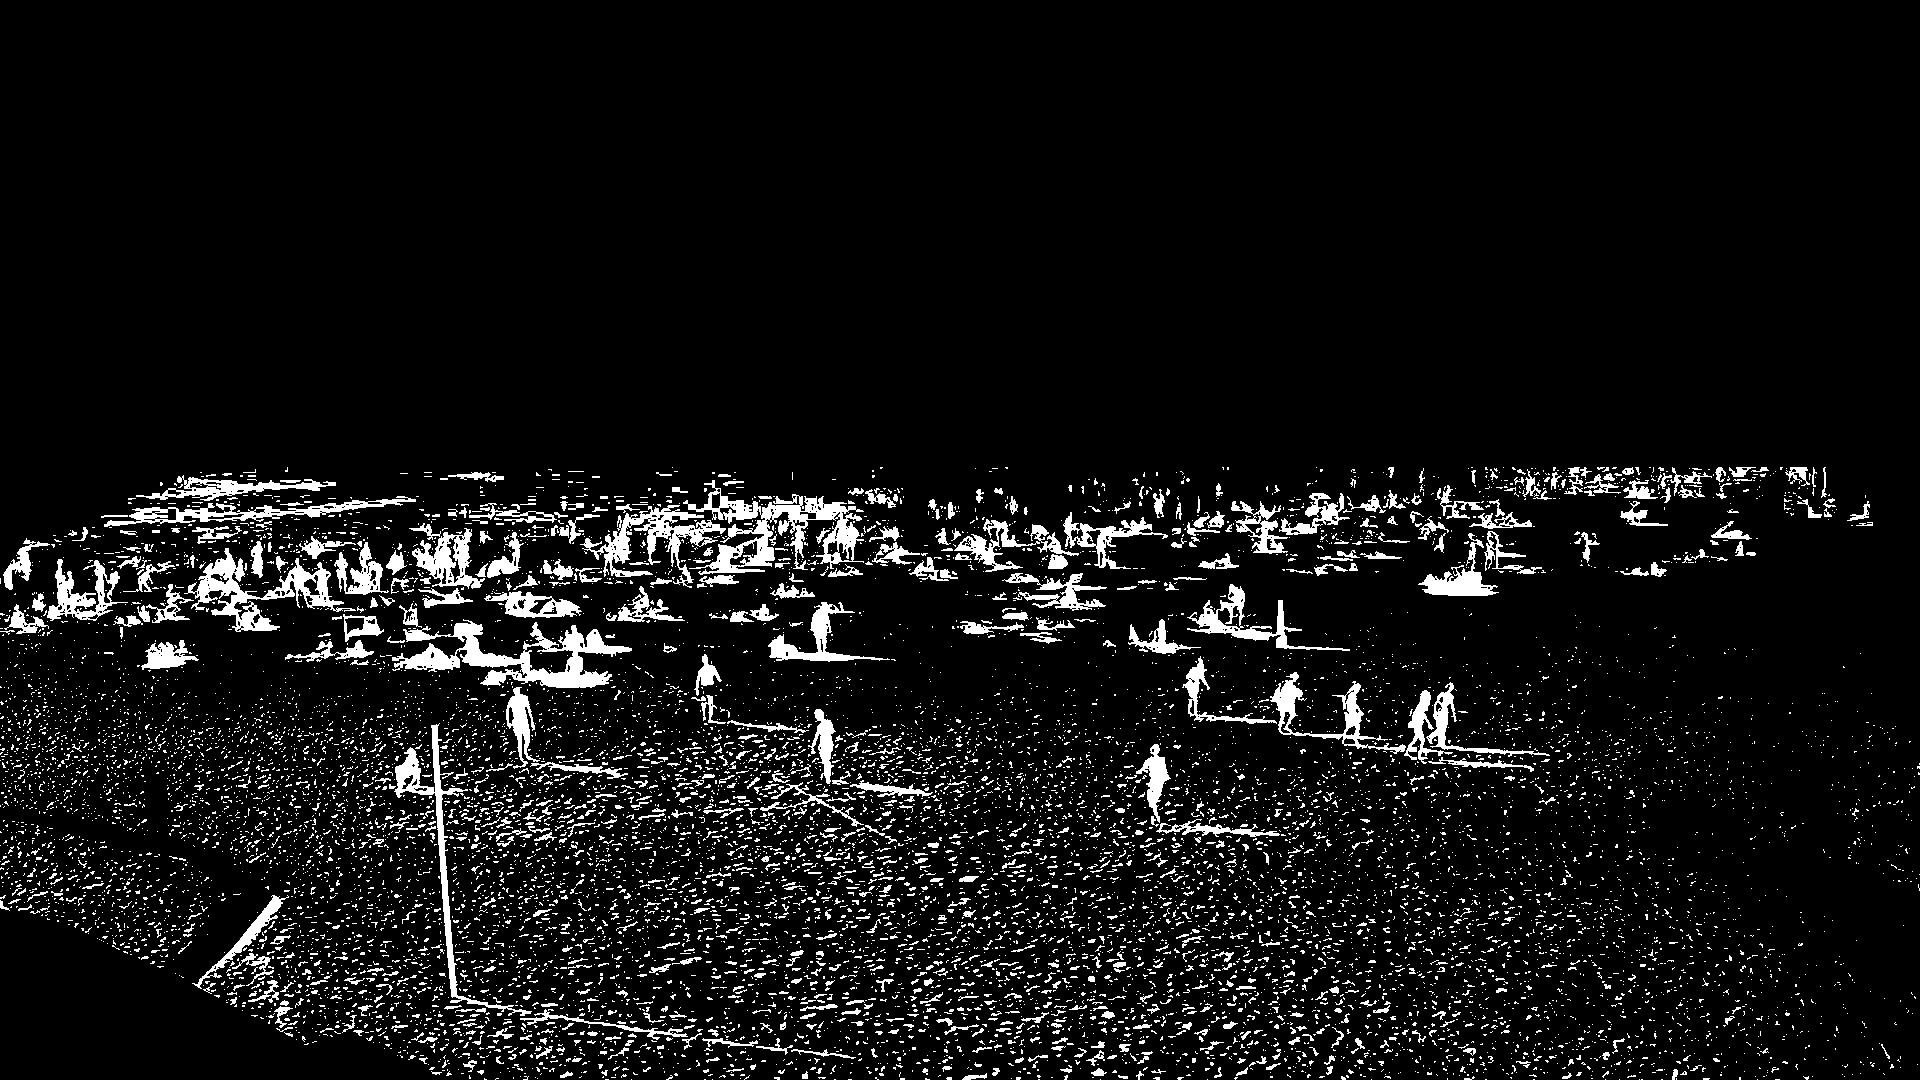
\includegraphics[width=\textwidth]{img/OTSU_sub_arena.jpg}
            \caption{Image substracting the empty beach image}
            \label{fig:y equals x}
        \end{subfigure}

        \begin{subfigure}[b]{0.3\textwidth}
            \centering
            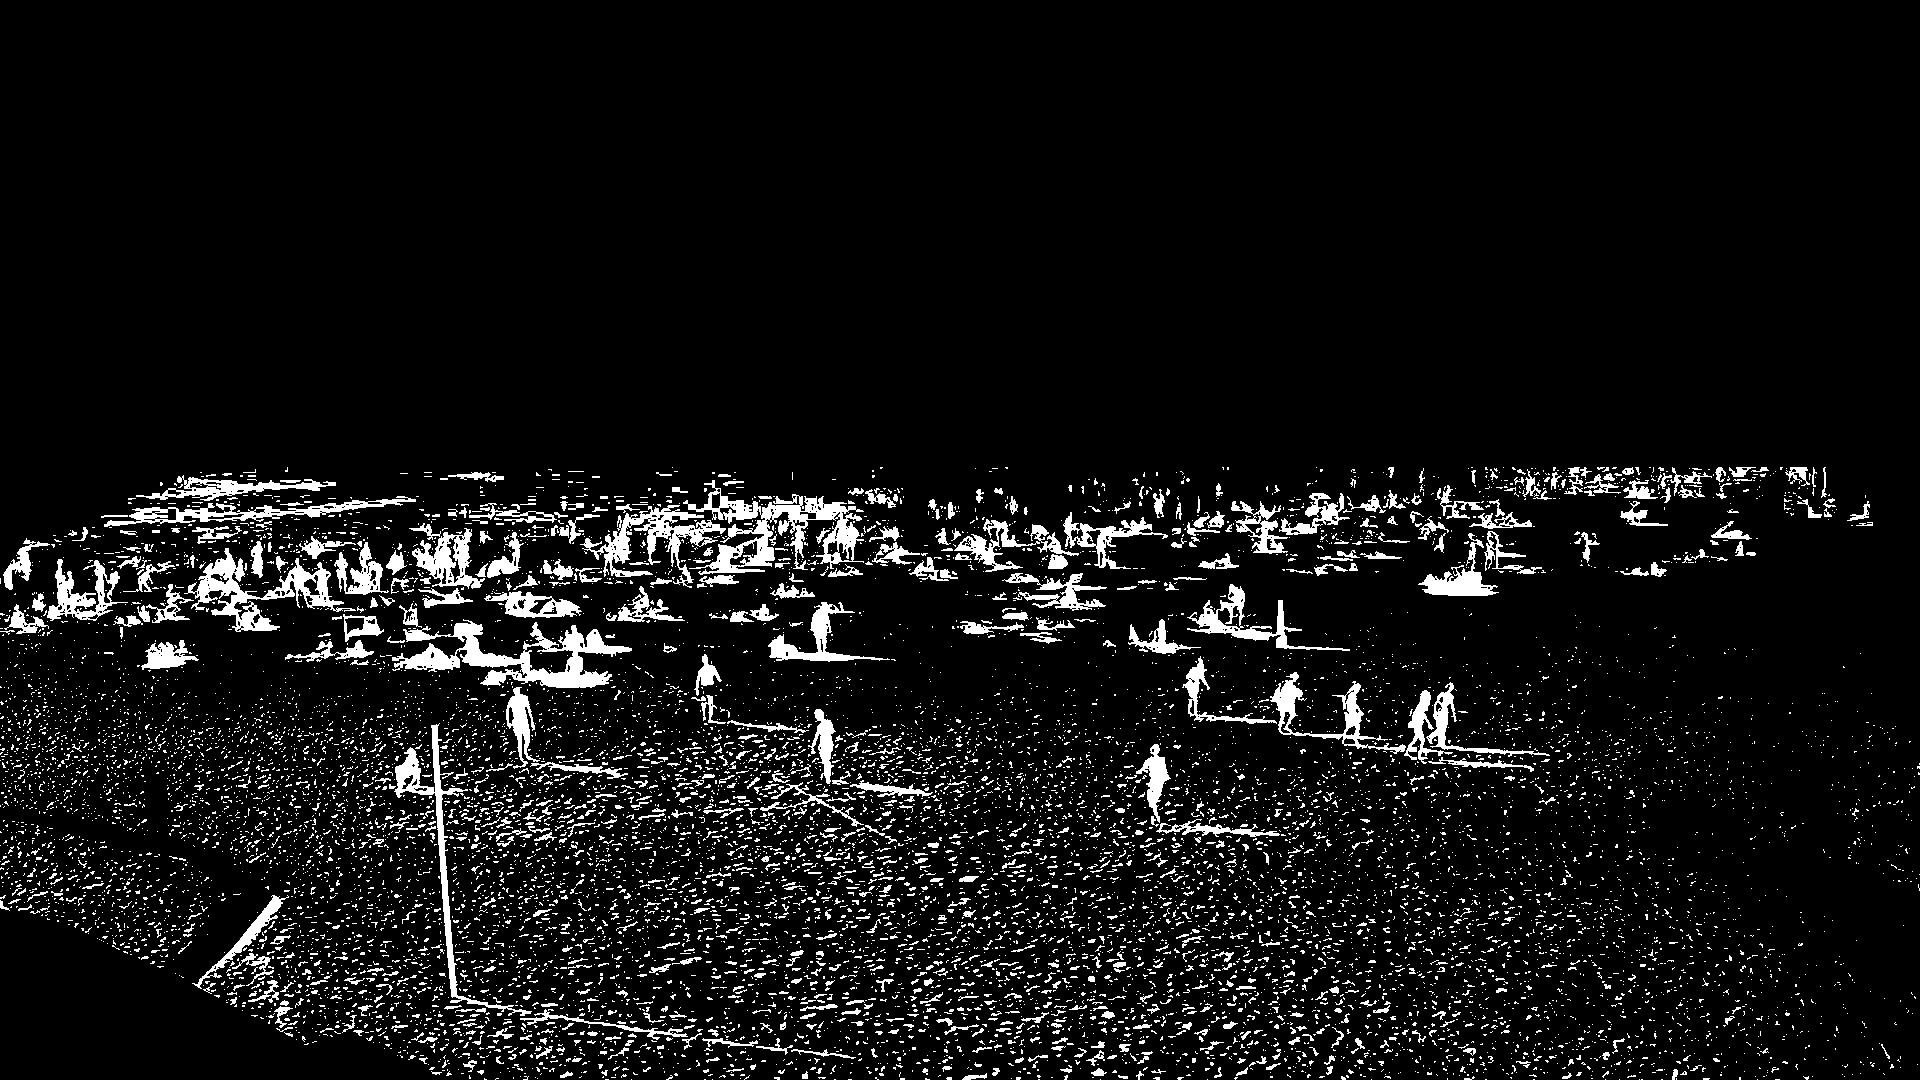
\includegraphics[width=\textwidth]{img/OTSU_sub_arena.jpg}
            \caption{sub}
            \label{fig:y equals x}
        \end{subfigure}
    \end{figure}
\end{comment}

\begin{figure}[h]
    \centering
    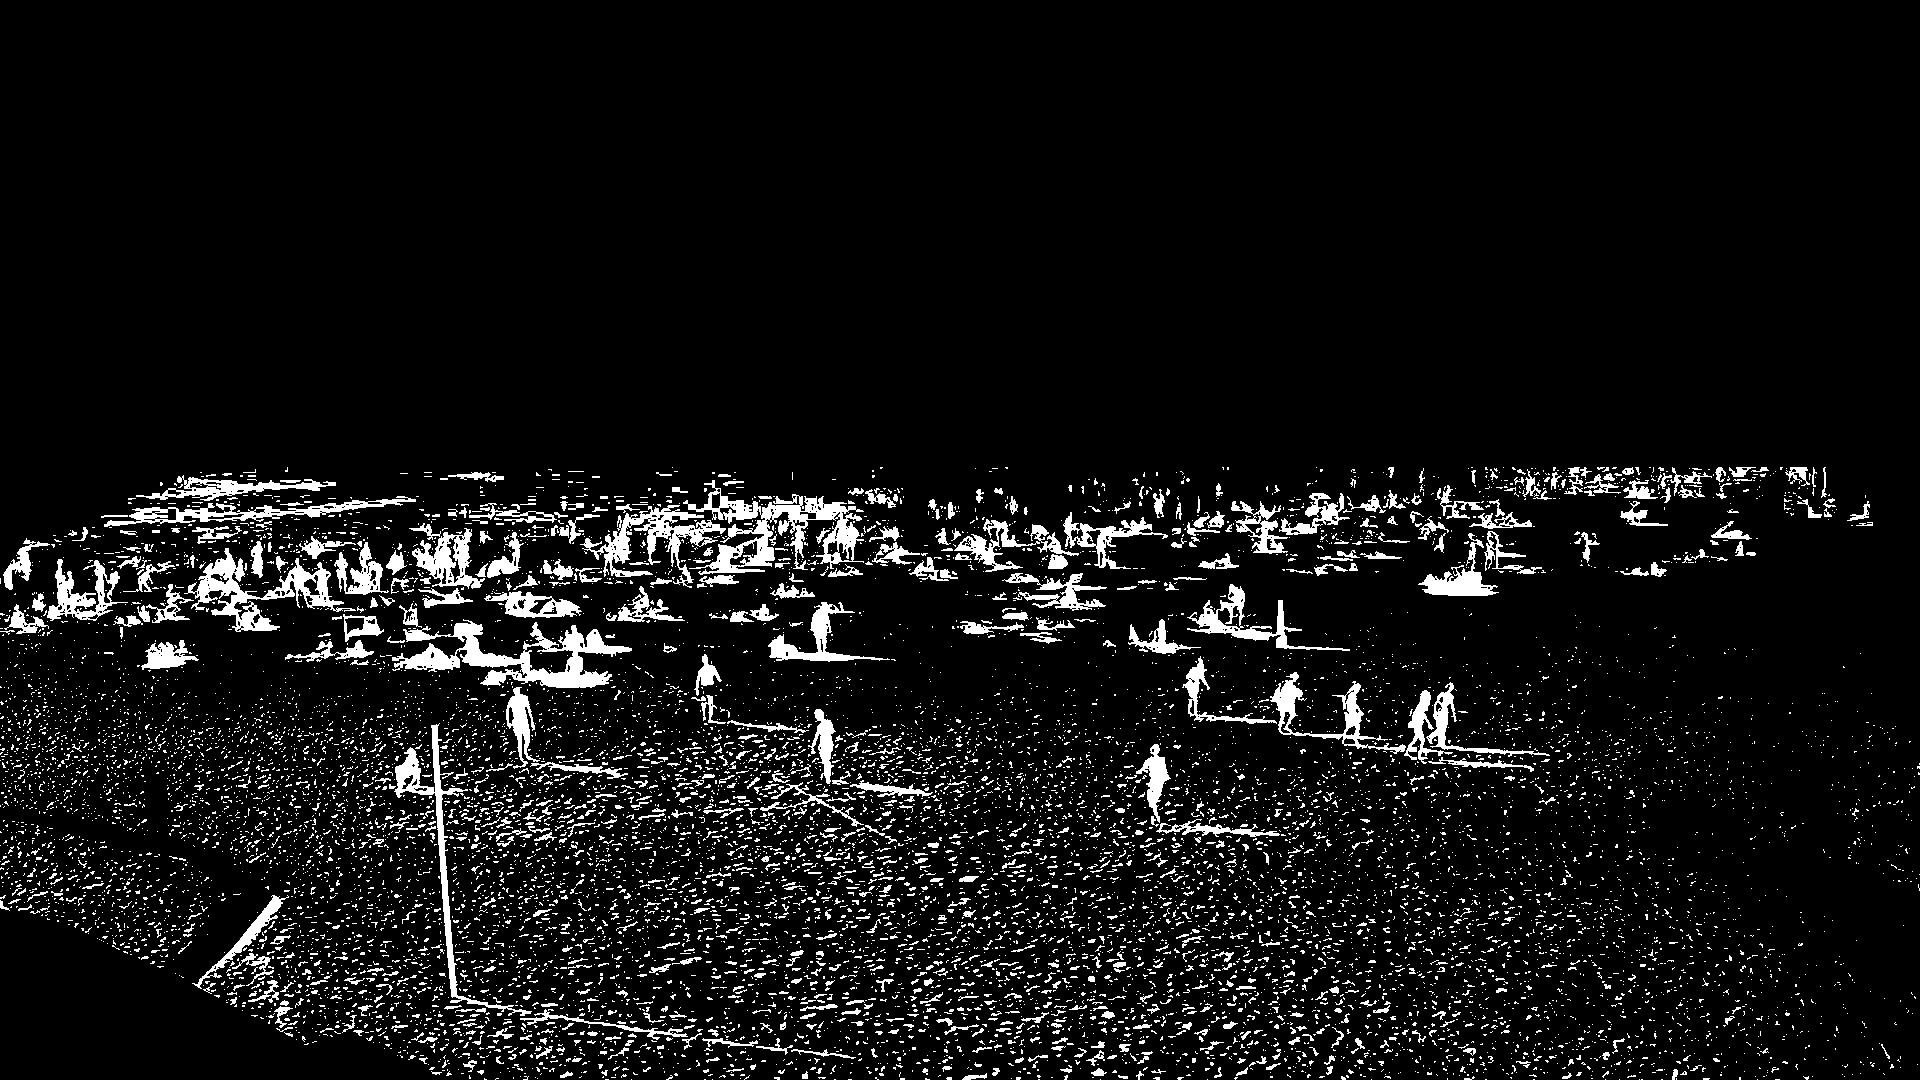
\includegraphics[width=\textwidth]{img/OTSU_sub_arena.jpg}
    \caption{Binarized image using OTSU and the empty beach image}
    \label{fig:y equals x}
\end{figure}

\subsubsection{Image Averaging}



\subsubsection{Image Substraction}
%In the areas where there is a person, at the time of applying the image substraction, we will be  


\section{Gabor Filter}

%Think as Gabor as a Gaussian filter in 2D.


A band pass filter generated by a function of various parameters.

\begin{equation}
    filter(x,y;\sigma,\theta,\lambda,\gamma,\phi) = exp [ - \frac{x^2 - \gamma ^2 \cdot y^2}{2 \sigma^2} ] \cdot exp [ i (2 \pi \frac{x}{\lambda} + \phi) ] 
\end{equation}

% Large sigma on small feature you will miss
% Small sigma on ...

The parameters of ksize allows to select the size of our kernel filter, in case we are using a really big shape we will overlook details if the shapes are small. The same reasoning can be applyed with a small filter, may overlook shapes too big for it. Therefore, must be tested with different sizes to reach an idoneal spot, if your features are tiny or bigger, you have to take that in count.

If we are looking for \textbf{horizontal-like} features, applying an horizontal filter will allow us to maintain those characteristics and block the vertical ones and viceversa in the other cases.


\section{What form do the People have?}

In general the shapes that a person can describe may suffer alot of distorsion depending of the angle where the frame was took, the person posture, etc. Not always will be a perfet pose to the researchers to easily identify if an object is a person or not. There is no key shape that we could use, but we can try use common sense. The images gathered, are related to people moving standing up, swiming or just taking sunbathing.


\end{document}
